%%%%%%%%%%%%%%%%%%%%%%%%%%%%%%%%%%%%%%%%%%%%%%%%%%%%%%%%%%%%%%%%%%%%%%%%%%%%%%%%%
%
%  Bachelor's/Master's Thesis       First Name      Last Name       Date
%  "Title"
%  Machine Learning and Data Analytics Lab, FAU Erlangen-Nuernberg
%
%%%%%%%%%%%%%%%%%%%%%%%%%%%%%%%%%%%%%%%%%%%%%%%%%%%%%%%%%%%%%%%%%%%%%%%%%%%%%%%%%
\documentclass{maddoc}
% ++ es werden keine underfull hboxes als Fehler ausgegeben,
%    da das ja nur heißt, dass die Seite noch nicht ganz voll ist
\hbadness=10000

% load the bibliography file
\addbibresource{bibliography.bib}

% Nomenclature
%\usepackage[english]{nomencl}
%\makenomenclature

\usepackage{graphicx}
\usepackage{hhline} % for more flexible horizontal lines in tables

% Ensure that lualatex looks very similar to pdflatex
\setmainfont{texgyretermes}[
  UprightFont = *-regular ,
  BoldFont = *-bold ,
  ItalicFont = *-italic ,
  BoldItalicFont = *-bolditalic ,
  Extension = .otf ,
  Scale = 1.0 ]
\defaultfontfeatures{Ligatures=TeX}

\Titel{Sharing Medical Trial Data in Federated Gaia-X Data Spaces}

\ThesisType{Master's Thesis}
\StudyProgramme{Data Science}

\FirstName{Jan}
\LastName{Šimerda}
\Birthplace{Hradec Králové}
\DateOfBirth{01.08.1999}
\Advisors{Michael~Nissen,~M.~Sc., René~Raab,~M.~Sc., Dr.~med.~Tobias~Steigleder, Prof.~Dr.~Bjoern Eskofier}
\Start{01.03.2024}
\Ende{30.08.2024}
%\PartnerInstitute{Some Other University}

% The date on page iii is automatically set to the current date, but can be overwritten like this:
%\renewcommand{\todayPreamble}{30.05.2022}
% Use this file to define LaTeX macros and placeholders
\newcommand{\OurMethod}{Fancy Name} % example: use \OurMethod as a placeholder for a name that isn't finalized yet.

% define mathematical variables: 
% It's good practice to define variables at one place and add a nomenclature if you have a lot of mathematical variables. 
% This will also help you to keep track of your naming schema.
% Example: 
%\def\states{\vec{x}}           \nomenclature[x]{$\states$}{State vector}

% define chapterabstract
\makeatletter
\newenvironment{chapterabstract}{\hfill\begin{minipage}{\dimexpr\textwidth-0.5cm}\itshape}{\end{minipage}\vskip 0.5cm\par\@afterindentfalse\@afterheading}
\makeatother


\pagenumbering{roman}

\begin{document}
\begin{center}
\bfseries
Übersicht
\normalfont
\end{center}
Deutsche Zusammenfassung (German Summary)

\vspace{5.0cm}

\begin{center}
\bfseries
Abstract
\normalfont
\end{center}
English Summary

% Print a table fo contents
\tableofcontents
\cleardoublepage

% Nomenclature
% \addcontentsline{toc}{chapter}{Nomenclature}
%\null\newpage
%\printnomenclature[4em]
%\cleardoublepage

% start arabic page numbers
\pagenumbering{arabic}

% CONTENT
% Here we include the actual content of the thesis.
% Feel free to add/remove/rename the files and include statements according to your needs.
% Each file should start with a \chapter{Title} command


% introduction
%---------------------------------------------------------------
\chapter{Introduction}\label{ch:introduction}

\section{Motivation}\label{sec:motivation}

The ongoing developments of hardware and software in information technology have caused electronic devices to steadily become more compact, lighter,
and more affordable for end customers.
Coupled with advancements in battery life, this trend has enabled the emergence of smart wearable devices,
with the first-ever market-produced ``smartwatches''
\footnote{The \textit{smartness} of the "Pulsar Calculator Watch" though was vastly different from our current
understanding of smart gadgets and was limited to arithmetic calculations.} appearing as early as 1975~\cite{ometov_survey_2021}.
Over time, this has ignited a growing interest in these devices among the general public, with now around
30\%~\cite{simon_kemp_rise_2023} of internet users owning a smartwatch or a smart wristband.

The hype around consumer-available wearable devices didn't leave the healthcare industry untouched.
Even though digital technologies have been successfully used in clinical setting for many years, the recent advances in
hardware and analytic capabilities have caused an explosion of interest in the use of digital technologies to
facilitate data collection in clinical trials~\cite{clay_impact_2017}.

The use of wearable technology in medical trials can potentially offer numerous benefits compared to the
traditional data collection approach.
These include --- but are not limited to --- longitudinal data measurement, out of clinic use, reduced cost, treatment response monitoring and improved data quality~\cite{munos_mobile_2016}.

The deployment of smart wearable devices in clinical trials along with their continuous recording capabilities results in significant increases in data volume~\cite{munos_mobile_2016}.
This may extend the possibilities of using deep learning, where the requirement for the size of a training dataset is increased, to analyze this data.

The increase in generated data volume presents an opportunity to exchange this data with other researchers or institutions, which can further reduce the cost of research.

This thesis examines the feasibility of using a Gaia-X-compliant solution to perform this exchange.
\textit{Gaia-X}~\cite{gaiax} is an initiative that emerged in 2019 in the EU and whose goal is to govern how data, digital services and infrastructure are exchanged in a decentralized federated environment.
This initiative does this by publishing specifications, parties must follow in order to participate.
Alongside the specifications, they also provide a reference implementation of the software services needed to run a Gaia-X federation under the project name Gaia-X Federation Services~\cite{gxfs}.
This includes mainly the framework facilitating data and software transactions and other useful tools, for example, a credential manager or data exchange logger.

\section{Purpose}\label{sec:purpose}

While the initiative already emerged in 2019, saw a continued increase in the number of members, lighthouse projects and national hubs, and was made publicly available in 2023.
There have also been reports of implementation delays, lack of agility, excessive bureaucracy and concerns about the market readiness of Gaia-X~\cite{say_gaia-x_2024},~\cite{noauthor_inside_2021},~\cite{eichberger_why_2021}.
The purpose of this thesis is to determine the feasibility of exchanging healthcare data via Gaia-X compliant processes.
This is done through the development of a Gaia-X-compliant module for data exchange in an existing framework Carecentive~\cite{carecentive}.
The exact research questions this thesis seeks to answer are outlined in Table~\ref{tab:research-questions}.

\begin{table}
    \centering
    {\renewcommand{\arraystretch}{1.7}
        \begin{tabular}{ p{4cm}|p{11cm} }
            Research Question 1 & Is it feasible to share healthcare data in Gaia-X Data Spaces?\\
            \hhline{--}
            Research Question 2 & What are the technical challenges in implementing Gaia-X-compliant software?
        \end{tabular}
    }
    \caption{Research Questions}
    \label{tab:research-questions}
\end{table}

\section{Outline}\label{sec:outline}

This section concludes the first chapter, which clarifies the motivation, purpose of this thesis, the research questions and finally the outline.
Next up, we provide the fundamentals of federated data and services architectures in Chapter~\ref{ch:fundamentals}.
The next chapter --- Chapter~\ref{ch:related-work} --- then follows up with a deep dive on literature related to the topic of this thesis.
The Chapter~\ref{ch:gaia-x-concepts} elaborates on the concepts used in the Gaia-X ecosystem in greater detail than in Chapter~\ref{ch:fundamentals}.
The Chapter~\ref{ch:methods} serves to clarify the methods of this work used to answer the research questions stated in this chapter.
The Chapter~\ref{ch:results} states the results of this work, which are then discussed in Chapter~\ref{ch:discussion}.
Lastly, Chapter~\ref{ch:conclusion} wraps up this thesis and provides a conclusion.

\clearpage


% Fundamentals
%---------------------------------------------------------------

\chapter{Fundamentals}\label{ch:fundamentals}

\begin{chapterabstract}
    In this chapter, we will introduce readers to the fundamentals of federated infrastructure with emphasis on data exchange and see how they compare to centralized architectures.
    The next part will focus directly on Gaia-X as a federated infrastructure representative.
    We will go over its vision, the means to achieve them, their organizational structure and fundamental concepts.
\end{chapterabstract}

\section{Federated Data Infrastructures}\label{sec:federated-data-infrastructures}

Federated infrastructures for data storage are such infrastructures, which do not pool data in a central data store, but instead independent federations of data providers are set up~\cite{otto_federated_2022}.
Instead of relying on a central data silo, data providers publish their offerings in a publicly searchable catalogue along with its metadata, terms and conditions, usage policies, etc.
After consumers find an offer they are interested in, they communicate with the data producer directly (P2P) via a data connector.

The advantages of federated data infrastructures are numerous; they can be more flexible than centralized solutions, which means they could cater to the needs and requirements of more diverse groups of people~\cite{raab_federated_2023}.
Federated architectures can also be more fault resilient than their centralized counterparts as a single node failure doesn't impact the whole network.
Since federated data infrastructures (also called ``Data Spaces'') don't require data to be transferred to a central location, the mere fact that they can be exchanged closer to source can increase data privacy and lower the risk of leaks.

However, the concept of Data Spaces is not without its downsides.
Centralized solutions have the edge over Data Spaces in terms of simplicity; the existence of multiple federations leads to an increased need of interoperability to reduce the increased effort of having to communicate with multiple parties.

\section{About Gaia-X}\label{sec:about-gaia-x}

\textbf{Gaia-X} is the initiative led by the ``Gaia-X Association AISBL'' organization.
The association was registered as an \textit{international non-profit association} \textit{(French: Association Internationale sans but lucratif)} in Belgium in January 2021 and is funded privately.
It was founded by \textit{22} companies and organizations in \textit{January 2021}, but at the time of writing (January 2024), the association has over \textit{350} members from backgrounds like data infrastructure providers, IT startups research institutions and business associations. % TODO: update before completing the thesis
Additionally, representatives from business, politics, academia, research, technology, policy, government, and science from Europe and beyond cooperate with the \textit{Gaia-X Association AISBL} in their mission.
The association claims to have no business interest~\cite{gaiax}.

\section{Goal}\label{sec:gaia-x-goal}

The goal of the \textbf{Gaia-X} initiative is to enable exchange of data and services in a \textit{safe} and \textit{trustworthy} environment~\cite{gaiax}.
The coveted outcome is a federated system connecting many service and data providers and users together in an environment that is \textit{interoperable} \textit{transparent}, \textit{open}, \textit{secure}, and respects \textit{data rights} and \textit{EU regulations}.

\section{Structure}\label{sec:the-structure}

The organisational structure of the ``Gaia-X Association AISBL'' is well-defined and transparent~\cite{gaiax}.
The topmost body of the \textit{association} is the \textbf{General Assembly}.
It is composed of all the members of the \textit{association} and has complete authority to carry out the objectives of the \textit{Gaia-X initiative}.

Under the \textbf{General Assembly} are the boards \em \textit{Governmental Advisory Board}, \textit{General Advisory Board} and the \textit{Board of Directors}.
The \textbf{Board of Directors} is elected by the \textbf{General Assembly} and is headed by a Chairperson and Vice-Chairperson.
Its purpose is to decide on important matters regarding the \textit{Gaia-X Association}.

Next up is the \textbf{Management Board} and its chairs \em \textit{Policy Rules Committee}, \textit{Data Spaces Business Committee}, and the \textit{Technical Committee}.
Each of the committees also has its own \textit{Working Group}.
The \textbf{Management Board} is appointed by the \textit{Board of Directors} and is composed of the Chief Executive Officer (CEO), the Chief Operating Officer (COO), the Chief Technical Officer (CTO), the Digital Communications Director and the Head of Finance and Administration.
Its purpose is the management of daily activities of \textit{Gaia-X Association}.

\begin{figure}
    \centering
    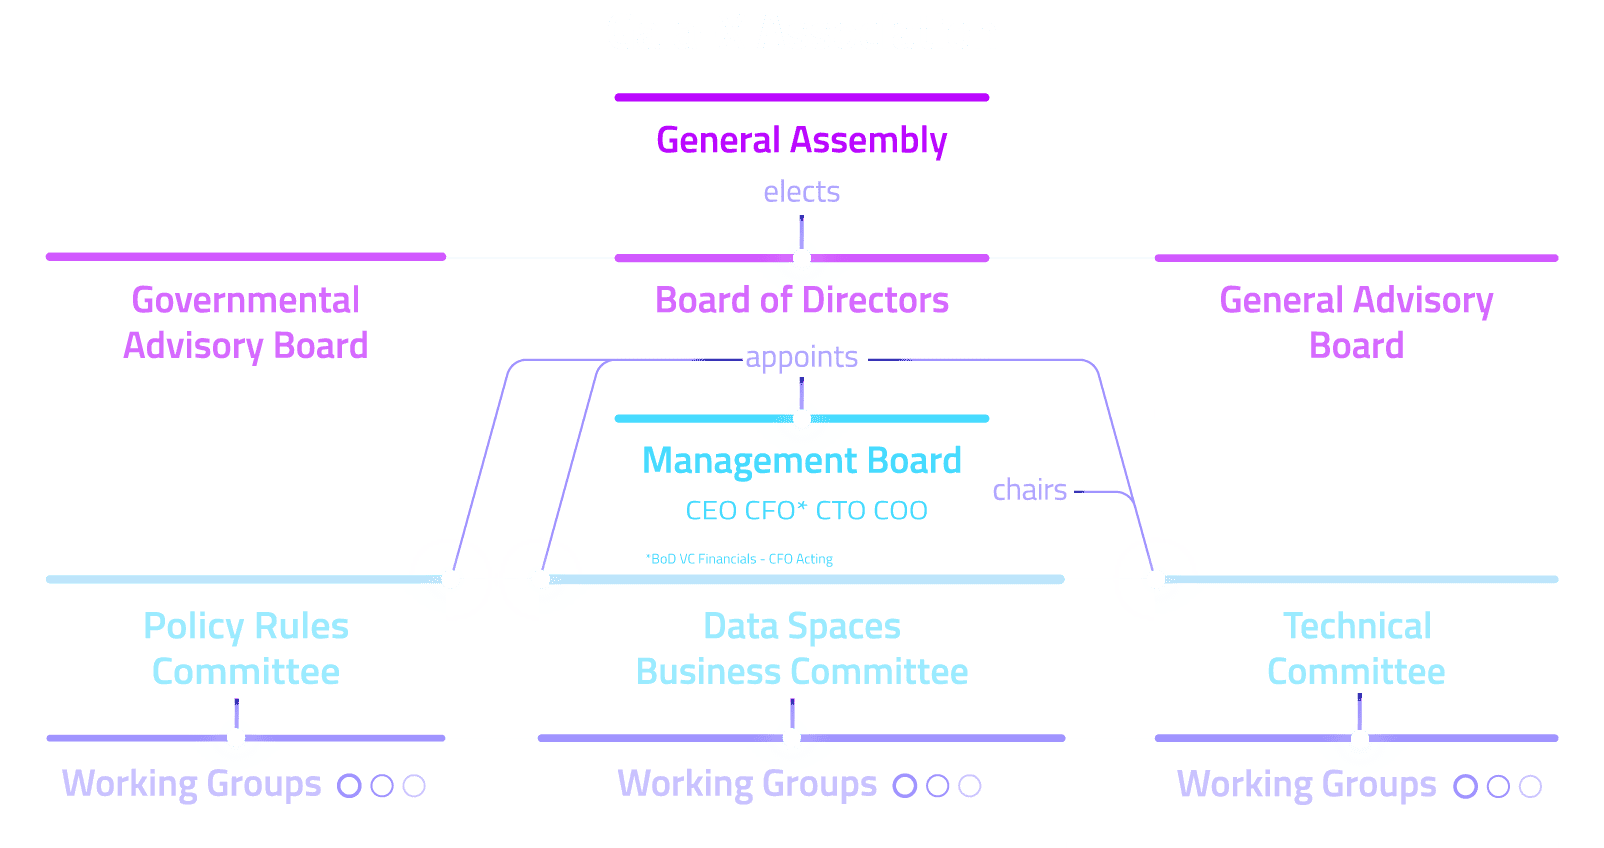
\includegraphics[width=\textwidth]{figures/management-board-structure.png}
    \caption{Organisational structure of the Gaia-X Association~\cite{gaiax}}\label{fig:organisational-board-structure}
\end{figure}

\subsection{Data Spaces Business Committee}\label{subsec:data-spaces-business-committee}

The \textit{Data Spaces Business Committee (DSBC)} focuses on collecting \textit{economic}, \textit{functional}, \textit{operational} and \textit{legal} requirements that facilitate seamless collaboration and interconnection between \textit{Data Spaces}, \textit{Ecosystems}, \textit{Lighthouse Projects\footnote{A lighthouse project is a high-impact, innovative initiative that serves as a model for others, demonstrating leadership and setting a benchmark within an industry or organization.}} and respective \textit{Hubs}~\cite{gaiax}. % FIXME: Data Spaces, Ecosystems, Lighthouse Projects and Hubs not defined yet
Furthermore, the \textit{DSBC} supports the creation of Data Spaces by third parties across Europe and beyond.

\subsection{Policy Rules Committee}\label{subsec:policy-rules-committee}

The \textit{Policy Rules Committee (PRC)} exists to translate the guiding principles of the Gaia-X initiative (\textit{transparency}, \textit{data protection}, \textit{cyber-security}, \textit{portability}, \textit{openness},~\ldots) into High-Level Objectives and to preserve the added value of the \textit{Gaia-X ecosystem}~\cite{gaiax}.
The additional role of the \textit{PRC} is to monitor, integrate and define the relationship with EU regulations and external standards.
The Committee guides and delivers the \textit{Gaia-X Trust Framework}, \textit{Gaia-X Policy Rules and Labelling Document} (formerly Policy Rules Document and Gaia-X Labelling Criteria).
These deliverables are provided by the Committee's three \textit{Working Groups} (WG).
\begin{itemize}
    \item \textbf{Labels \& Qualification} WG:~provides the \textit{Gaia-X Labelling Framework} and prepares the ``Gaia-X Policy Rules and Labelling Document'' together with the \textit{Policy Rules Document} WG
    \item \textbf{Policy Rules Document} WG:~defines \textit{High-Level Objectives} and prepares the ``Gaia-X Policy Rules and Labelling Document'' together with the \textit{Policy Rules Document} WG
    \item \textbf{Compliance} WG:~provides the \textit{Gaia-X Trust Framework}, representing the reference document for the Gaia-X compliance, providing the compulsory set of rules of the Gaia-X Ecosystem
\end{itemize}

\subsection{Technical Committee}\label{subsec:technical-committee}

The purpose of the \textit{Technical Committee (TC)} is to define and implement the technological vision of the \textit{Gaia-X initiative}~\cite{gaiax}.
It is in charge of transforming the high-level objectives of Gaia-X and requirements collected from other Committees and Gaia-X members into the \textit{technology roadmap} and is accountable for its contributors.
The Committee drafts and delivers the Gaia-X \textit{Architecture Document}, \textit{technical specifications} and related \textit{reference implementation}.
These deliverables are provided by the Committee's two \textit{Working Groups} (WG).
\begin{itemize}
    \item \textbf{Architecture} WG:~drafts the ``Gaia-X Architecture Document'', which describes the founding concepts of the \textit{Gaia-X Ecosystem}
    \item \textbf{Service Characteristics} WG:~specifies the Schema for the Self-Descriptions of Providers, their Service Offerings, and the Resources they are composed of
\end{itemize}

\begin{figure}
    \centering
    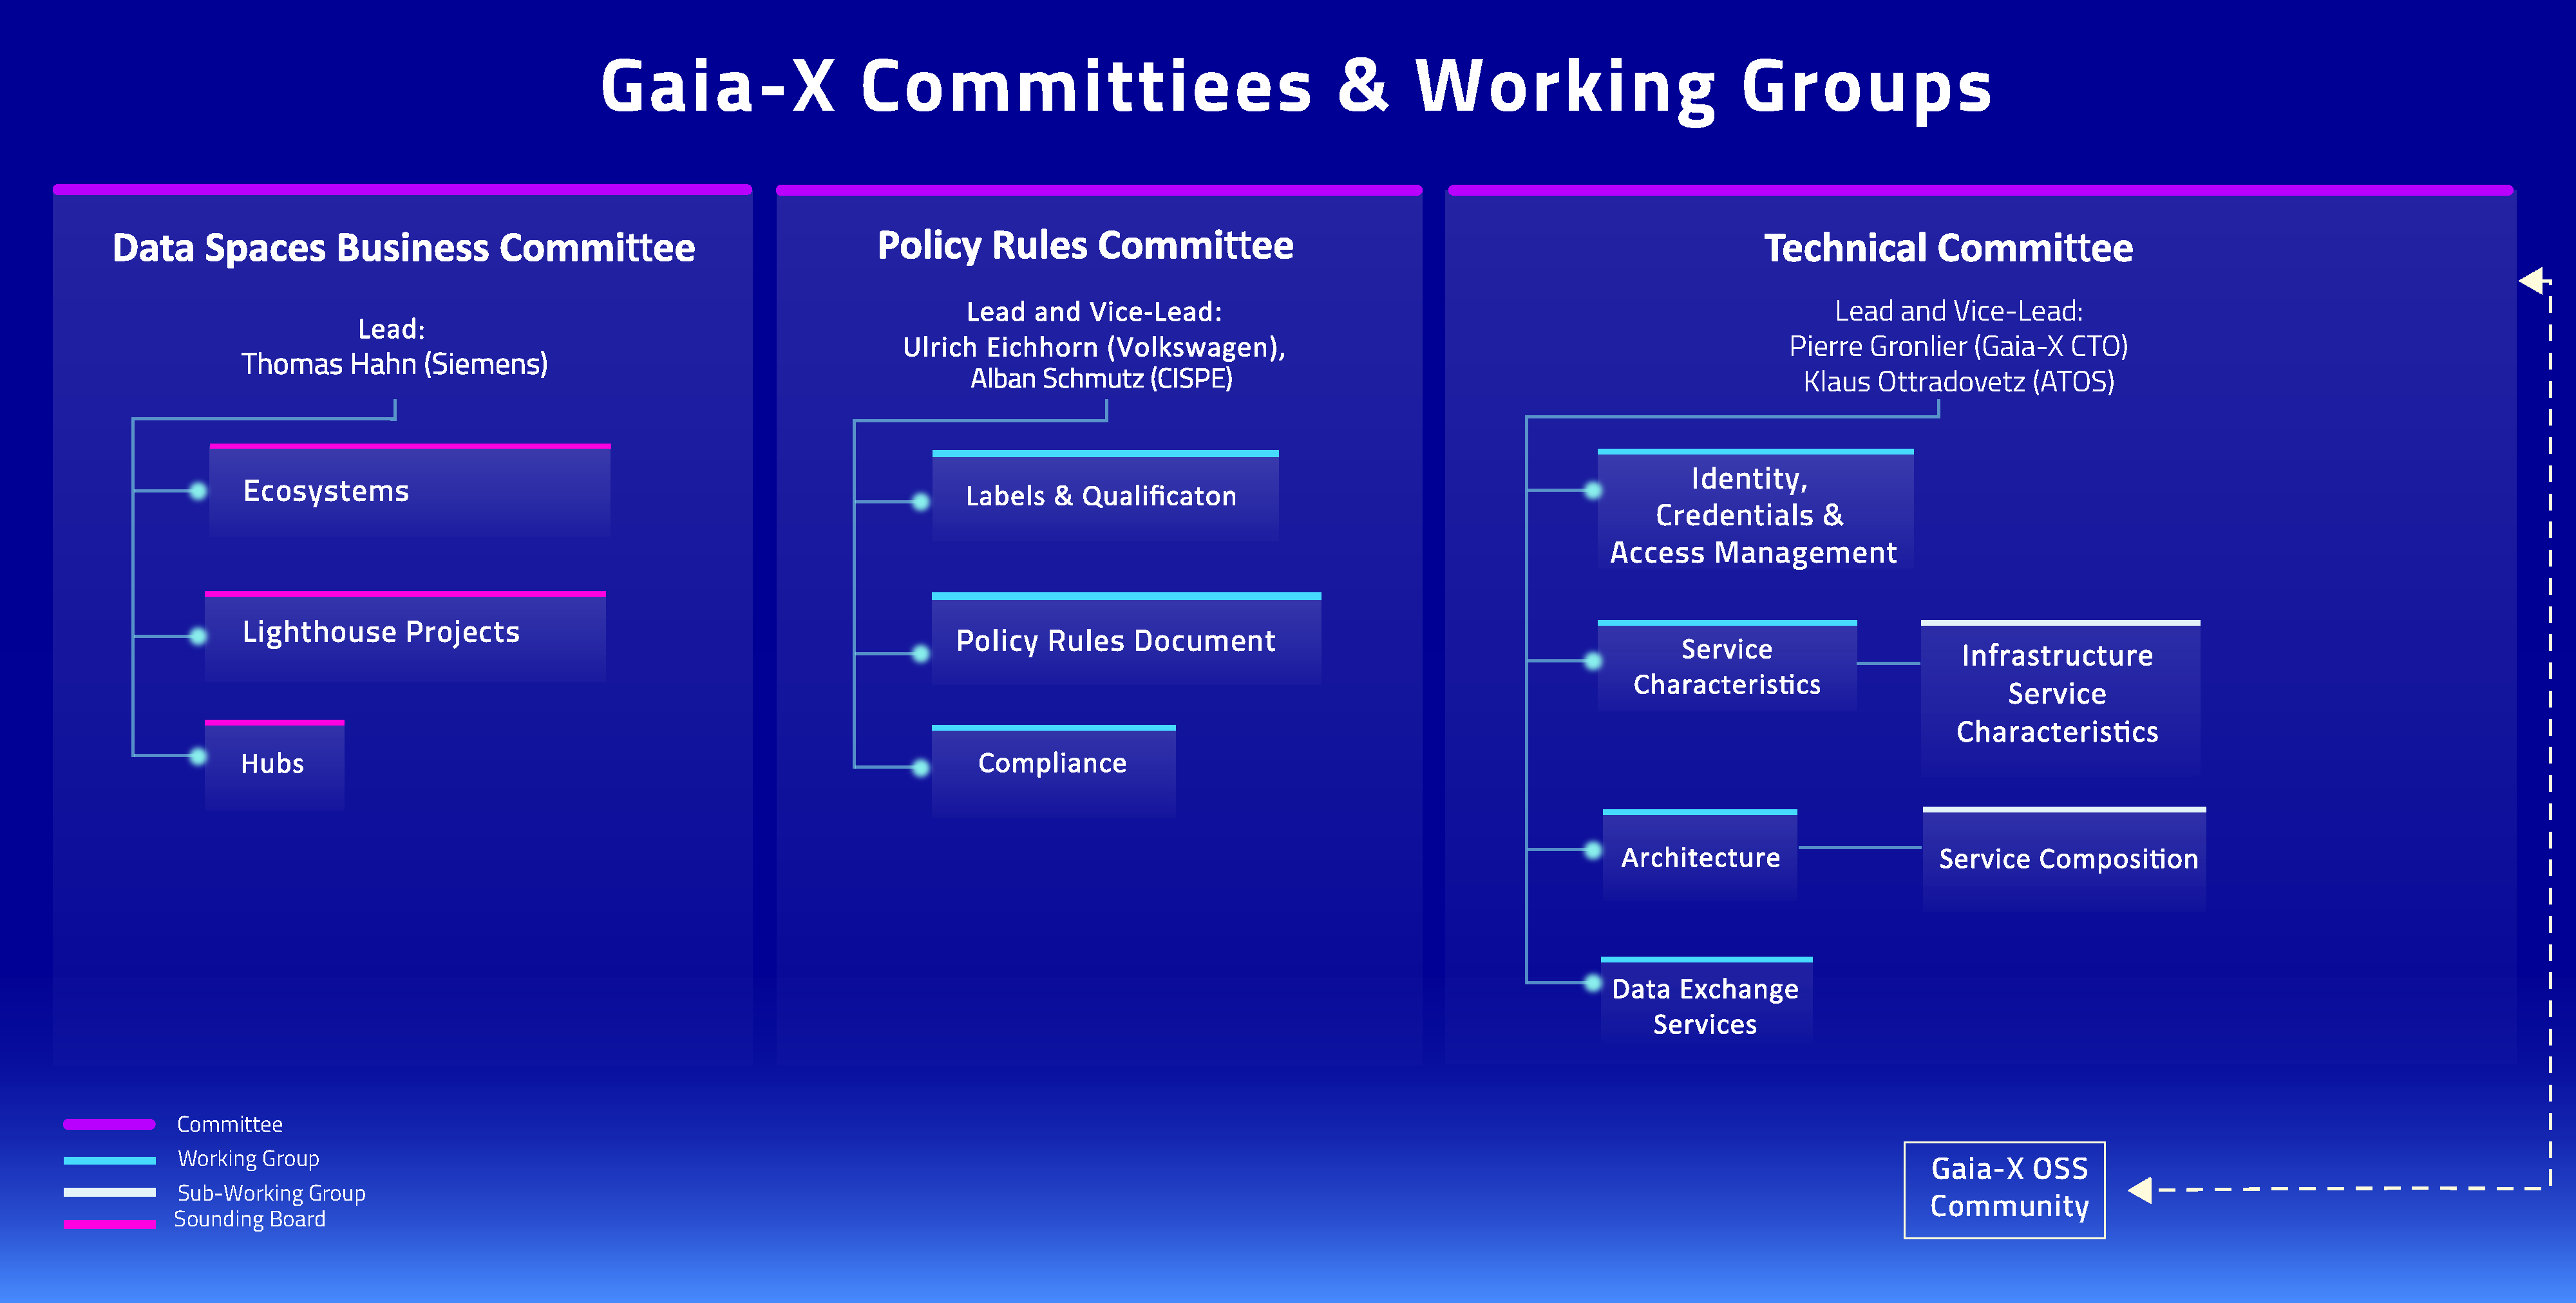
\includegraphics[width=\textwidth]{figures/committees-and-working-groups.pdf}
    \caption{Organisational structure Committees and their Working Groups~\cite{gaiax}}\label{fig:organisational-committees-structure}
\end{figure}

\begin{figure}
    \centering
    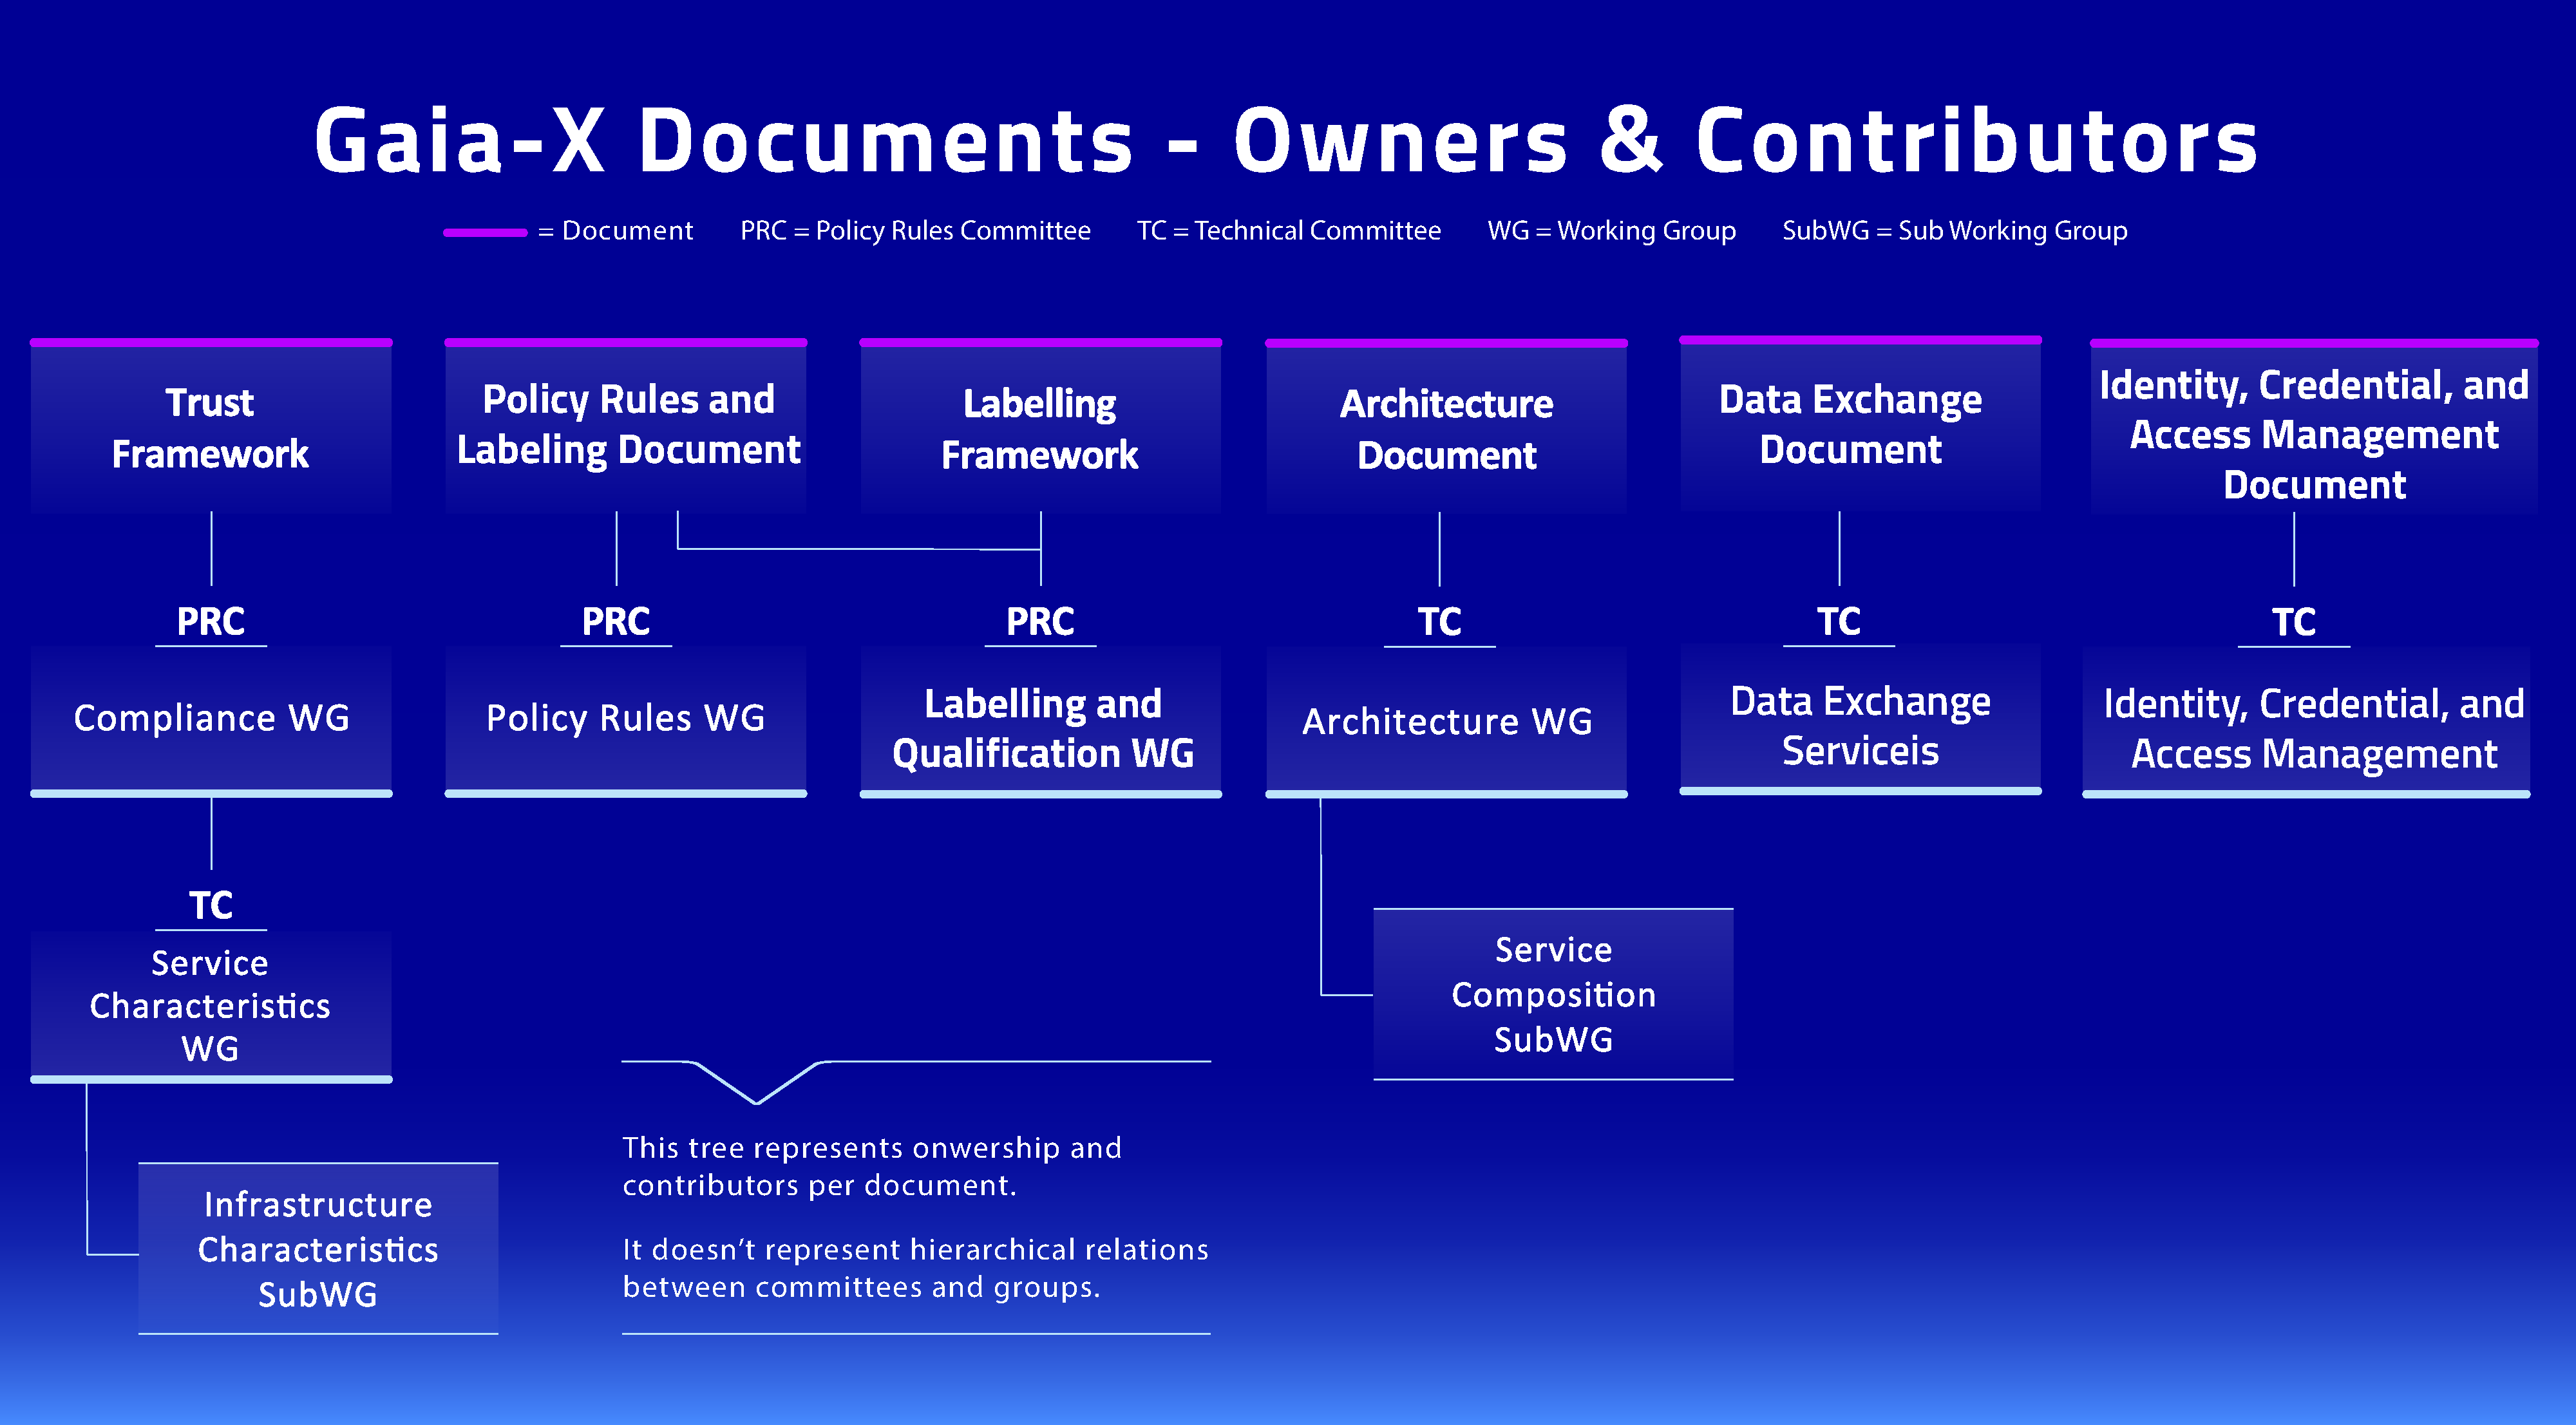
\includegraphics[width=\textwidth]{figures/committees-owners-and-contributors.pdf}
    \caption{Gaia-X Documents - Owners \& Contributors~\cite{gaiax}}\label{fig:gaiax-documents-owners-and-contributors}
\end{figure}

\section{Gaia-X Framework}\label{sec:gaia-x-framework}

Gaia-X Framework (also known as X-Model) is a set of the main deliverable of the initiative and serves to achieve the goal of exchange of digital services, data and cloud storage.
The Gaia-X Association delivers the documents containing formal specifications and requirements for parties wanting to participate in the Gaia-x ecosystem.
These can be categorized into three broad pillars:
\begin{itemize}
    \item Compliance: Decentralized services to enable objective and measurable trust
    \item Federation: Interoperable \& portable Sector or Cross-Sector datasets and services
    \item Data/Service exchange: Anchored contract rules for access and data usage
\end{itemize}

Once the formal specifications are ready, it is the task of the Gaia-X Federation Services (GXFS) project to convert the specifications into freely accessible, open-source software~\cite{gxfs}.
The software is mainly used by Gaia-X participants to support the creation of federations and to provide helpful tools like a logging service or cryptographic libraries.

\begin{figure}
    \centering
    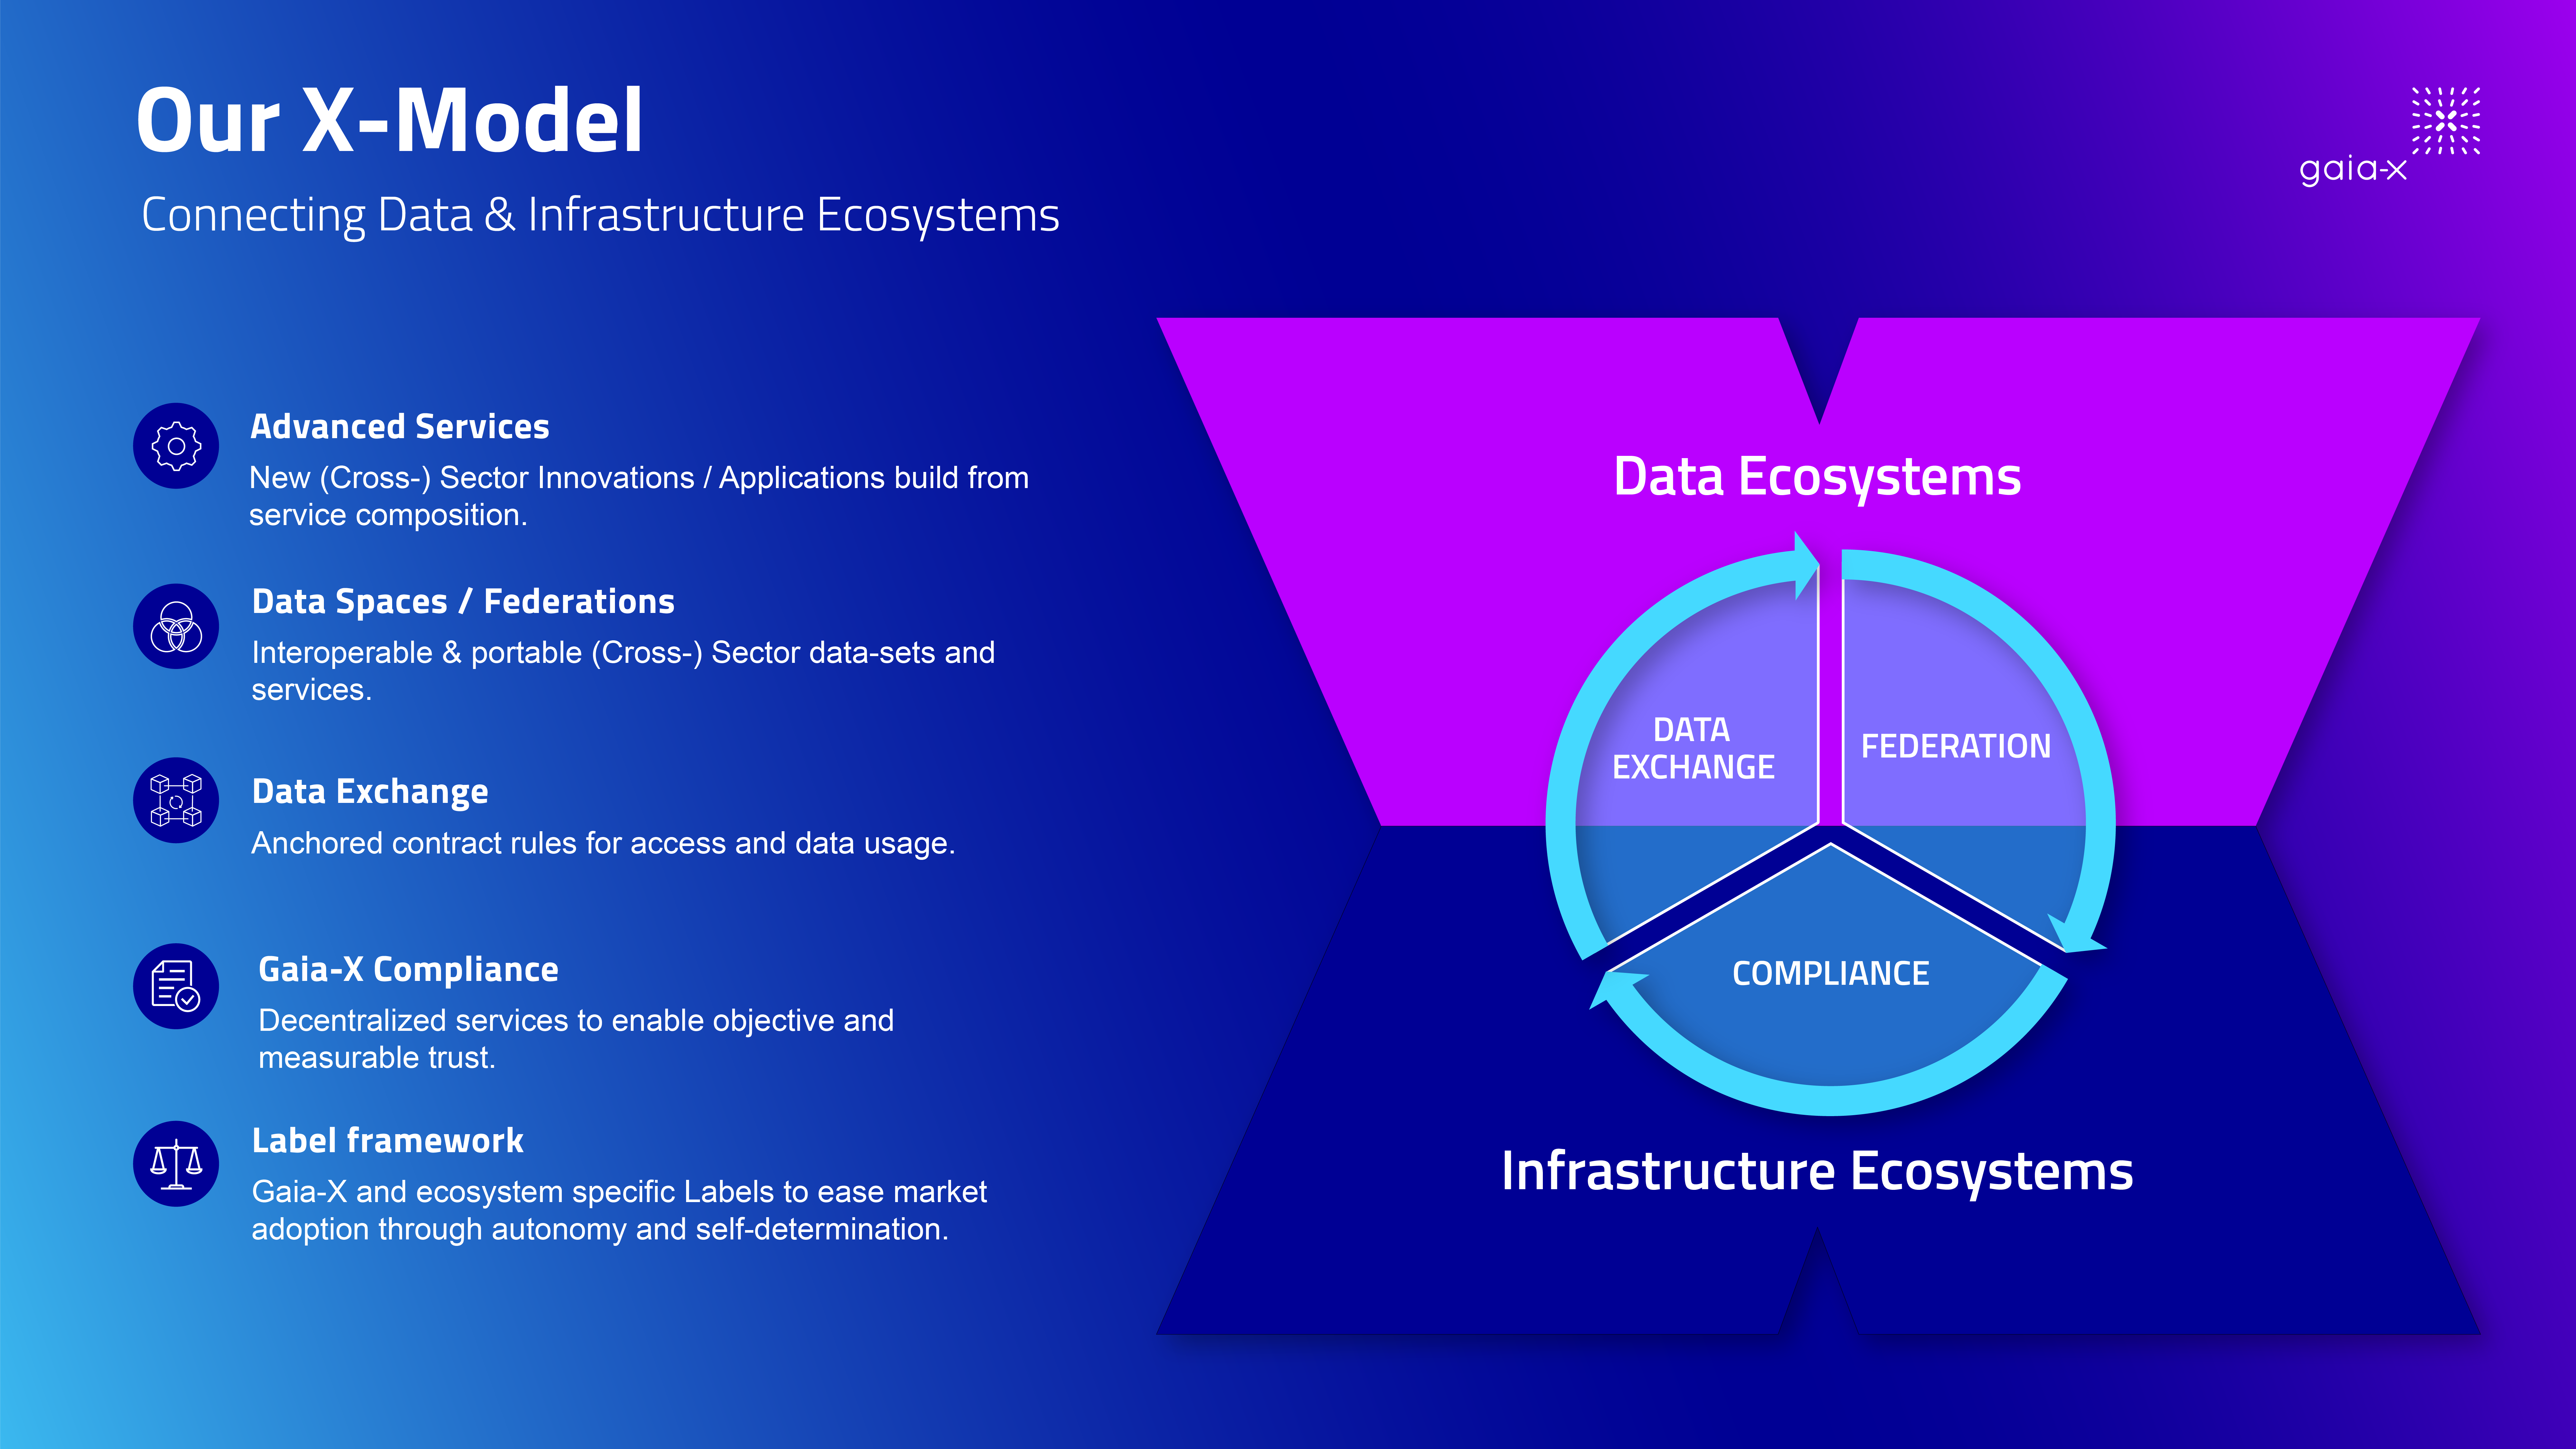
\includegraphics[width=\textwidth]{figures/x-model.png}
    \caption{Gaia-X Framework~\cite{gaiax}}\label{fig:gaiax-x-model}
\end{figure}

\subsection{Policy Rules Conformity Document}\label{subsec:policy-rules-conformity-document}

This document defines high-level objectives of and safeguards the added value and principles of the Gaia-X Ecosystem~\cite{gaiax_policy_rules}.
The policy rules aim to establish clear controls that reflect the core European values of Gaia-X: openness, transparency, data protection, security, and portability.
Basic Conformity sets the minimum requirements for participation in the Gaia-X Ecosystem.
Optional Label levels specify additional criteria and measures, such as certifications, to provide higher assurance and trust, emphasizing European values and complying with EU/EEA legislation.
These initial Labels are expandable, allowing for new Labels to meet sector-specific or regional needs in the future.
Compliance with these policy rules can be demonstrated through adherence to established standards, certifications, and codes of conduct.

The latest version of the document at the time of writing this thesis is 22.10.

\subsection{Architecture document}\label{subsec:architecture-document}

This document outlines the core components of the Gaia-X Trust Framework and explains their interrelationships within the Gaia-X model (see~figure~\ref{fig:gaiax-x-model}) at a functional level~\cite{gaiax_architecture_document}.
Since the Gaia-X Association collaborates with various partners to develop infrastructure and data-driven ecosystems, additionally, this document details how the Gaia-X Trust Framework integrates with implementations of Infrastructure and Data Space-specific services.

The latest version of the document at the time of writing this thesis is 23.10.

\subsection{Trust Framework}\label{subsec:trust-framework}

This document defines the minimum set of rules to be part of the Gaia-X Ecosystem~\cite{gaiax_trust_framework}.
These rules include common governance and basic interoperability across individual ecosystems.
The Gaia-X Trust Framework operationalizes the requirements outlined in Gaia-X documents, such as the Policy Rules, the Labeling Document and the Architecture Document. % FIXME: Labeling document not available on the Gaia-X framework knowlegbase page, reevaluate whether to keep this mention
The latter, in particular, enables federated and interoperable Gaia-X ecosystems.
The framework relies on verifiable credentials and linked data representations as key components for its future operations.

Trusted information must be accessible in machine-readable formats, and when such formats are unavailable, Gaia-X will establish processes to convert this information.
This is essential for federating trusted statements within the Gaia-X ecosystem and for developing mechanisms to reassess the validity of claims within the Trust Framework.
The compliance process, a set of automated and versioned computable rules, ensures this document will also be versioned.
This version of the Gaia-X Trust Framework document supersedes all previous versions.

The latest version of the document at the time of writing this thesis is 22.10.

\subsection{Identity, Credential \& Access Management}\label{subsec:identity-credential-&-access-management}

This document outlines the components of ``Authorization \& Authentication'' that will provide essential functionalities for authorization, access management, and authentication, along with related services, to Gaia-X Participants~\cite{gaiax_identity_and_access_management}.
These functionalities are intended to facilitate participation in the secure environment of the Gaia-X ecosystem.
This document does not address the replacement of an existing IAM System within a Gaia-X participant's environment or its operation therein.

The latest version of the document at the time of writing this thesis is 22.10.

\subsection{Data Exchange services}\label{subsec:data-exchange-services}

This document states the specifications of \textit{Data Exchange Services} including high-level architecture and key requirements for data values, trust and compliance~\cite{gaiax_data_exchange_document}.

The latest version of the document at the time of writing this thesis is 23.11.

\section{Concepts}\label{sec:concepts}

\subsection{Self-Descriptions}\label{subsec:self-descriptions}
The Gaia-X Framework is centered around so-called \textit{self-descriptions}, which are based on the \textit{W3C Verifiable Credentials Data Model} --- digital, machine-readable credentials containing cryptographical proof from the issuer, in a \textit{JSON-LD} format, which can be linked-up together (e.g., a dataset credential can contain an attribute referencing the credential of the owner of the data).
Self-Descriptions are the cornerstone used to describe all the necessary objects required for participation inside a Gaia-X federation.
These include mainly a \textit{Participant}, \textit{Service Offering} and \textit{Resource}.

\subsection{Ecosystems}\label{subsec:ecosystems}

Gaia-X ecosystems are groups whose goal is to support the creation and development of Data Spaces and projects in different business sectors like Health, Infrastructure, Tourism, etc~\cite{gaiax}. % TODO: define dataspace

The ecosystems aim to create a breeding ground for the creation of new Data Spaces by sharing knowledge, collecting cross-country use-cases and giving Gaia-X Association members the opportunity to network, collaborate and identify open standards related to specific domains.
The cooperation between ecosystems is supported by the Gaia-X Data Space Business Committee to ensure the development and application of Gaia-X deliverables in specific domains.

Currently established ecosystems include the following sectors: Aerospace, Agriculture, Tourism, Education, Energy, Finance, Geoinformation, Health, Manufacturing, Media, Mobility, Public Sector, Smart Cities, Smart Living, Construction and Logistics.

\subsection{Hubs}\label{subsec:hubs}

Apart from Ecosystems, Gaia-X Hubs also exist as groups of companies supporting the needs of Data Spaces~\cite{gaiax}.
Unlike Ecosystems, they act on a regional or country basis.
They serve as the central contact point of contact for interested parties in each country.
They cooperate with the Gaia-X Association in creating expertise and resources, setting up data spaces, and working on use cases.
They can be thought of as think tanks, where concrete data spaces are investigated, designed and implemented.

The hubs are tightly connected to local governments, which allows them to propose solutions in line with the strategic political initiatives and aligned with the goals of the Gaia-X Association and other European hubs~\cite{gaiax}.
In summary, the Gaia-X Hubs have the following objectives:
\begin{itemize}
    \item Act as a local ambassador for Gaia-X
    \item Identify territory specific needs and high priority data spaces
    \item Collaborate with other hubs to develop common pan-European data spaces
    \item Make Gaia-X real identifying projects and creating Gaia-X services in the market
    \item Help local governments implementing RRF in the most effective way adopting Gaia-X solutions
    \item Promote the participation of new members in the association
\end{itemize}

\clearpage


% Related Work
%---------------------------------------------------------------

\chapter{Related Work}\label{ch:related-work}

\begin{chapterabstract}
    This chapter covers a review of literature related to the topics of digital sovereignty, federated infrastructure, data spaces, and finally the Gaia-X initiative itself.
    The review offers insight into the feasibility of the Gaia-X vision, its upsides and potential challenges as well as their mitigation strategies and possible use-cases.
    Selected topics are covered in technical, legal, security, and geopolitical standpoints.
    The chapter ends with a conclusion drawn from the review literature.
\end{chapterabstract}

\section{Data Spaces and Federated Architectures}\label{sec:data-spaces-and-federated-architectures}
%TODO: shorten TOC subsection names
\subsection{Designing Data Spaces}\label{subsec:designing-data-spaces}

The book ``Designing Data Spaces -- The Ecosystem Approach to Competitive Advantage'' by Boris Otto et al., explores frameworks and technologies behind data spaces, focusing on initiatives like Gaia-X and the International Data Spaces (IDS)~\cite{designing_dataspaces}.
It emphasizes the importance of security and data sovereignty; \textit{``natural person’s or corporate entity’s capability of being entirely self-determined with regard to its data''}~\cite{designing_dataspaces} in the context of data exchange for innovation across sectors.
The book discusses the development, principles, technical, and governance aspects of data spaces, highlighting the need for harmonized approaches and public-private partnerships in Europe.

The Chapter~4 -- Role of Gaia-X in the European Data Space Ecosystem, provides a comprehensive introduction to Gaia-X, explaining its objectives, principles, and the economic and business impact of data.
Gaia-X's role in creating a federated, interoperable and secure data infrastructure for industries such as finance, energy, automotive, and health is examined, showing its broad applicability.
The book is a helpful resource for understanding Gaia-X, offering insights into its impact on secure data exchange and innovation.

A noteworthy section of the chapter is about the measuring of success of Gaia-X.
It mentions the goal of doubling the cloud usage in Europe within 4--5 years as well as the announced contribution of 1.2~B\char"20AC~ by the European Commission for the creation of data spaces. % TODO: consider evaluating these metrics for the current state of Gaia-X

\subsection{Project Gaia-X: A Federated Data Infrastructure as the Cradle of a Vibrant European Ecosystem}\label{subsec:project-gaia-x:-a-federated-data-infrastructure-as-the-cradle-of-a-vibrant-european-ecosystem}

``Project Gaia-X: A Federated Data Infrastructure for Europe'' is a publication by the German Federal Ministry for Economic Affairs and Energy (BMWi) --- now named Federal Ministry for Economic Affairs and Climate Action (BMWK) --- which published at the inception of the project in 2019.
The publication presents the Gaia-X project fueled by the vision of a secure, transparent, and sovereign data infrastructure for Europe~\cite{project_gaia_x}.
Motivated by the dependency on non-European cloud providers and the risks of data sovereignty loss, the ministry presents the project aims to create an open digital ecosystem where data can be securely shared and utilized across various sectors, including public administration, healthcare, and enterprises.

The project seeks to integrate existing cloud and edge computing services into a unified system that enhances interoperability and reduces complexity.
This federated approach allows for seamless switching between providers, minimizing lock-in effects and fostering competition.
According to authors, small and medium-sized enterprises (SMEs), in particular, stand to benefit from easier adoption and broader access to cloud technologies.

The publication mentions plans for establishing a governing entity, developing a robust reference architecture --- steps which are bring carried out at the moment --- and setting standards to ensure economic viability and sustainability.
By doing so, Gaia-X aims to uphold European values and standards in the global data economy, promoting innovation and economic growth while ensuring data sovereignty

\subsection{Gaia-X and IDS}\label{subsec:gaia-x-and-ids}

The position paper ``Gaia-X and IDS'' by the International Data Spaces Association (IDSA) examines how the International Data Spaces (IDS) Reference Architecture Model (IDS-RAM) aligns with Gaia-X principles~\cite{gaiax_and_ids}.
Gaia-X, a newer initiative, aims to create a federated cloud infrastructure that promotes data sovereignty, interoperability, and innovation across sectors in Europe.
IDS, established in 2015, offers a mature framework for secure data exchange and sovereignty.

Gaia-X focuses on overcoming cloud landscape fragmentation and legal uncertainties, supporting seamless data exchange through standardized models.
IDS provides a framework with roles like data owners and consumers and includes a certification scheme for trust and security.

The paper highlights that Gaia-X and IDS are complementary.
Gaia-X's infrastructure benefits from IDS's data sovereignty and security capabilities.
Integration areas include digital identities, certification, self-description, usage control, and trustworthy runtime environments.
For example, Gaia-X's Federated Catalogue can use IDS components, and IDS's Clearing House can enhance Gaia-X's data services.

Future steps for Gaia-X include establishing the Gaia-X Foundation and launching Federation services, with continued collaboration with IDS to support sovereign digital ecosystems in Europe.

\subsection{The Adoption of Data Spaces: Drivers Toward Federated Data Sharing}\label{subsec:the-adoption-of-data-spaces:-drivers-toward-federated-data-sharing}

The paper ``The Adoption of Data Spaces: Drivers Toward Federated Data Sharing'' by Andreas Hutterer and Barbara Krumay explores factors influencing the adoption of data spaces for federated data sharing among organizations~\cite{adoption_of_data_spaces}.
These spaces address issues of data sovereignty, trust, and value, which hinder interorganizational data sharing.

Through interviews with 28 experts, the study identifies twelve key drivers: controllable complexity, cost clarity, data sovereignty, ecosystem governance, ecosystem readiness, interoperability, mature technology, regulatory certainty, security, technology competence, transparency, and trust.
These drivers help overcome technical and organizational challenges.

The findings emphasize the need for a holistic approach, highlighting the relevance to the Gaia-X initiative.
By addressing these drivers, Gaia-X can enhance competitiveness and innovation in the digital economy through improved data exchange and collaboration.
The study provides a foundation for future research and practical implementation of data spaces.


\subsection{Foundation Data Space Models: Bridging the Artificial Intelligence and Data Ecosystems}\label{subsec:foundation-data-space-models:-bridging-the-artificial-intelligence-and-data-ecosystems}

The vision paper ``Foundation Data Space Models: Bridging the Artificial Intelligence and Data Ecosystems'' by Edward Curry et al., published by the \textit{IEEE} discusses integrating foundation models with data-sharing infrastructures called data spaces~\cite{foundation_data_space_models}.
Foundation models, pre-trained on extensive data and fine-tuned for specific tasks, are transforming AI. Data spaces, crucial to the European Data Strategy, ensure high-quality data sharing.

The authors propose Foundation Data Space Models (FDSM), where data spaces offer training data and governance, and foundation models provide advanced services.
This integration addresses challenges like data availability, trust, governance, and handling multimodal data.

The paper outlines a lifecycle for FDSM, covering data creation, sharing, deployment, discovery, maintenance, improvement, training, adaptation, and service deployment, aiming for efficient integration of foundation models into data spaces.

The work calls for research on FDSM, focusing on interoperability, multimodal data handling, robustness, and ethics, to advance European data spaces and AI ecosystems.

\section{Health Data and European Health Data Space (EHDS)}\label{sec:health-data-and-european-health-data-space}

\subsection{Security Engineering of Patient-Centered Health Care Information Systems in Peer-to-Peer Environments}\label{subsec:security-engineering-of-patient-centered-health-care-information-systems-in-peer-to-peer-environments}

The paper ``Security and Privacy Issues in Peer-to-Peer Patient-Centered Health Care Information Systems'' by Abdullahi Yari et al., published in the \textit{Journal of Medical Internet Research} in November 2021, examines the use of peer-to-peer (P2P) networks in personal health systems (PHSs) to decentralize health data management~\cite{security_engineering_p2p_environments}.
This approach aims to empower patients and improve health information exchange efficiency.
The study highlights the advantages of P2P networks, such as eliminating central points of failure, enabling direct resource sharing, and allowing self-organization.

Real-world examples, like the \textit{e-toile} P2P framework in Geneva and the \textit{PEPP-PT} COVID-19 contact tracing system, demonstrate the practical benefits of P2P networks in healthcare.
However, the paper also addresses significant security and privacy challenges, including vulnerabilities to snooping nodes, lack of content verification, network heterogeneity, and risks of disclosing sensitive information.
To mitigate these issues, the authors propose solutions like robust authentication protocols, trust and reputation systems, end-to-end encryption, and mobile agent-based intrusion detection systems.% TODO: consider the relevance of these solutions for Gaia-X

The study underscores the importance of ongoing research to ensure P2P PHSs can achieve their potential while maintaining high security and privacy standards.

\subsection{European Health Data Space}\label{subsec:european-health-data-space}

The paper ``European Health Data Space—An Opportunity Now to Grasp the Future of Data-Driven Healthcare'' by Denis Horgan et al., published in the \textit{Healthcare} journal explores how the European Health Data Space (EHDS) can revolutionize European healthcare by optimizing the use of health data~\cite{european_health_data_space}.
The EHDS aims to enhance healthcare delivery, patient outcomes, and research by improving data accessibility, privacy, and interoperability.
Key points include the EHDS's proposal for better access to health datasets for research and public health authorities.
The authors stress the need for strong data protection measures, compliance with European standards and governance to build public trust.

Key challenges highlighted include the need for supportive legislation, stakeholder engagement, and policies that balance data sharing with privacy concerns.
The EHDS represents a crucial step towards a more integrated and efficient healthcare system in Europe, offering valuable insights for advancing data-driven healthcare innovations.

\subsection{Federated electronic health records for the European Health Data Space}\label{subsec:federated-electronic-health-records-for-the-european-health-data-space}

The paper ``Federated electronic health records for the European Health Data Space'' by René Raab et al., published in \textit{The Lancet Digital Health} journal discusses the implementation of a federated architecture for electronic health records (EHRs) within the European Health Data Space (EHDS)~\cite{raab_federated_2023}.
The authors argue that while the EHDS aims to empower citizens by giving them access to and control over their health data, traditional centralized data storage systems pose significant privacy and security risks.
To mitigate these concerns, the paper proposes a decentralized model called ``federated personal health data spaces,'' which stores health data on personal devices or cloud servers under their control, rather than central servers solely managed by a provider.
The paper suggests for the proposed system to go beyond the storage of medical data and allow citizens to include wearable device, digital wellness and preventive care data.
Authors stress the need for the interoperability of the EHDS implementation to avoid a fragmented data landscape, leading to rejection from citizens and researchers alike.

The paper highlights the potential benefits of this model, including better patient outcomes, increased engagement with health data, and the facilitation of large-scale population studies.
The flexibility of the federated approach allows it to cater to diverse user needs, from those who prefer to manage their data independently to those who might delegate control to a trusted entity.

In conclusion, the proposed federated personal health data spaces offer a viable alternative to centralized data storage systems, aligning with the EHDS objectives while addressing privacy and security concerns.
This model not only empowers citizens but also fosters a more inclusive and transparent health data ecosystem, ultimately benefiting both individual healthcare and broader medical research initiatives.

\subsection{Federated learning of predictive models from federated Electronic Health Records}\label{subsec:federated-learning-of-predictive-models-from-federated-electronic-health-records}

The paper ``Federated Learning for Healthcare Informatics'' by Jie Xu et al., published in the \textit{Journal of Healthcare Informatics Research} examines how federated learning (FL) can address the challenges of using fragmented and sensitive healthcare data~\cite{federated_learning_for_healthcare_infromatics}.
FL allows decentralized data sources to collaboratively train machine learning models without sharing the data, preserving privacy and regulatory compliance.
Authors review reviews FL applications in healthcare, focusing on issues like data heterogeneity and communication efficiency.
Solutions include consensus methods and pluralistic approaches to manage diverse data sources, along with privacy measures such as secure multi-party computation and differential privacy.

Key healthcare applications include predictive modeling, phenotyping, and patient similarity learning.
FL has shown effectiveness in improving predictions for hospital readmissions and managing chronic diseases without compromising privacy.
In summary, FL offers a promising approach for collaborative, privacy-preserving healthcare analytics, enhancing patient outcomes and advancing research, with ongoing research needed to tackle technical challenges.

\subsection{Legal and technological aspects for the creation of a European Health Data Space}\label{subsec:legal-and-technological-aspects-for-the-creation-of-a-european-health-data-space}

The paper ``Legal and Technological Aspects for the Creation of a European Health Data Space'' by André Caravela Machado and Daniel Ferreira Polónia, published by the \textit{IEEE} discusses developing a European Health Data Space (EHDS)~\cite{legal_and_technological_aspects_of_ehds}.
It covers the legal and technological requirements for a unified data infrastructure in the EU.

From the legal standpoint, it examines GDPR implications, focusing on privacy, anonymization, and secondary use of health data, emphasizing the need for alignment with GDPR.
Technologically, it highlights data governance and quality, proposing a framework to balance data accessibility with privacy protections.

The paper stresses a harmonized approach among EU member states to enhance data sharing and interoperability, improving health outcomes and supporting advances in personalized medicine and healthcare efficiency.

In conclusion, the authors suggest mechanisms for individuals to control their health data access, ensuring compliance with privacy regulations.
Authors conclude the EHDS to be essential for leveraging data to improve healthcare and foster innovation in the European health sector.

\subsection{Sovereignly Donating Medical Data as a Patient: A Technical Approach}\label{subsec:sovereignly-donating-medical-data-as-a-patient:-a-technical-approach}

The paper ``Sovereignly Donating Medical Data as a Patient: A Technical Approach'' by Florian Lauf et al., proposes a system to enhance patient control over medical data donations for research~\cite{sovereignly_donating_medical_data}.
The authors introduce a patient portal where patients can view and select specific research projects to support, enhancing data sovereignty.

Integrating concepts from the Medical Informatics Initiative (MII), International Data Spaces (IDS), and MY DATA Control Technologies, the system uses IDS Connectors for secure data transfer and enforces patient choices through usage control policies.
This approach builds trust by providing transparency and control, ensuring interoperability with existing medical data standards like HL7 FHIR.

In the context of Gaia-X, the paper demonstrates principles of data sovereignty and secure data sharing, aligning with Gaia-X's goals of a federated and secure data infrastructure in Europe.
It showcases a practical application of Gaia-X's framework, promoting trust and control over data usage.

\section{Digital Sovereignty and EU Policies}\label{sec:digital-sovereignty-and-eu-policies}

\subsection{Digital Sovereignty in the EU: Challenges and Future Perspectives}\label{subsec:digital-sovereignty-in-the-eu:-challenges-and-future-perspectives}

The chapter ``Digital Sovereignty in the EU: Challenges and Future Perspectives'' by Edoardo Celeste published by the book \textit{Data Protection Beyond Borders} examines the concept of digital sovereignty in the European Union (EU)~\cite{dig_sovereignty_challenges}.
It highlights the EU's dependence on foreign technology companies, mainly from the US and China, and the associated risks to fundamental rights and geopolitical stability.

Celeste contextualizes digital sovereignty historically, noting its evolution from traditional notions of territorial control to encompass control over data and digital infrastructures in the digital age.
The paper discusses recent EU policies aimed at reducing reliance on non-European service providers by promoting local data storage and European digital services.
These initiatives, including Gaia-X, are part of the EU's effort to regain control over its data and protect its values and rights.

The paper also addresses the potential downsides of digital sovereignty, warning against a protectionist approach that could lead to internet fragmentation and international conflicts.
Celeste emphasizes the need for a balanced approach that fosters international cooperation while safeguarding the EU's strategic interests.

In conclusion, the paper argues for a pursuit of digital sovereignty that avoids isolationism and promotes global collaboration, ensuring the protection of fundamental rights and a secure, independent digital future for the EU.

\subsection{Europe's Quest for Digital Sovereignty: Gaia-X as a Case Study}\label{subsec:europe's-quest-for-digital-sovereignty:-gaia-x-as-a-case-study}

The paper ``Europe’s Quest for Digital Sovereignty: Gaia-X as a Case Study'' by Simona Autolitano and Agnieszka Pawlowska discusses Europe's efforts to achieve digital sovereignty through the Gaia-X project~\cite{europe_quest_for_digital_sovereignty}.
Authors mention the initiative's aspirations to establish a federated data infrastructure aligned with European values like data sovereignty and protection, reducing dependence on US and Chinese tech giants.

The authors highlight past national cloud initiatives, such as France’s Andromède and Germany’s Bundescloud, and their challenges, like the struggle to compete with foreign tech giants.
Gaia-X focuses on creating a secure, interoperable cloud ecosystem adhering to EU regulations like GDPR with the intent of fostering competition and innovation within Europe.

Despite its promise, Gaia-X faces risks, particularly from potential involvement of non-EU companies, which might dilute its goal of digital sovereignty.
The authors emphasize that Europe should leverage its regulatory strength to ensure the project's success and truly achieve digital independence.

\subsection{In Search of Digital Sovereignty and Strategic Autonomy}\label{subsec:in-search-of-digital-sovereignty-and-strategic-autonomy}

The paper ``In Search of Digital Sovereignty and Strategic Autonomy: Normative Power Europe to the Test of Its Geopolitical Ambitions'' by Dennis Broeders et al., published in the \textit{Journal of Common Market Studies} examines the EU's evolving concepts of digital sovereignty and strategic autonomy in the context of global geopolitics~\cite{digital_sovereignty_and_strategic_autonomy}.
The authors explore how the EU seeks to balance its strong regulatory and economic power with its ambitions to be a geopolitical player, particularly in the digital sphere.

The paper identifies three key trends: the use of internal market policies to exert geopolitical influence, the imposition of foreign policy goals on national markets, and the creation of hybrid digital policies that blend market, rights, and geopolitical concerns.
These trends highlight the EU's efforts to reduce its reliance on foreign technology and assert greater control over its digital infrastructure through projects like Gaia-X.

However, the authors warn that this push for digital sovereignty could create tensions between the EU’s traditional role as a normative power, focused on rights and market freedom, and its new geopolitical ambitions.
The lack of cohesion among EU member states and the risk of strategic discord further complicate this balance.

\subsection{The Discursive Struggle for Digital Sovereignty}\label{subsec:the-discursive-struggle-for-digital-sovereignty}

The paper ``The Discursive Struggle for Digital Sovereignty: Security, Economy, Rights and the Cloud Project Gaia-X'' by Rebecca A.-Nissen and Kristin A. Eggeling, published in the \textit{Journal of Common Market Studies} examines the conflicting interpretations of ``digital sovereignty'' within the EU, using the Gaia-X project as a case study~\cite{discursive_struggle_for_digital_sovereignty}.
The authors identify six distinct conceptions of digital sovereignty across three domains: security, economy, and rights.
These include views of digital sovereignty as ``strategic autonomy'' or ``cybersecurity'' in security, ``neo-mercantilism'' or ``market cosmopolitanism'' in the economy, and ``personal privacy'' or ``data ownership'' in the rights domain.

The paper argues that these varying interpretations create tension and ambiguity within the EU's digital policy.
The authors outline three potential future scenarios for the EU's digital sovereignty agenda: coexistence of multiple views (constitutional tolerance), dominance of one perspective (hegemony), or the collapse of the agenda due to internal contradictions.
The study underscores that this ambiguity could either bolster or undermine the EU's efforts to assert digital sovereignty on the global stage, making it a critical issue for the future of European digital governance.

\section{Data Mesh and Decentralized Data Management}\label{sec:data-mesh-and-decentralized-data-management}

\subsection{Data Mesh as Distributed Data Platform for Large Enterprise Companies}\label{subsec:data-mesh-as-distributed-data-platform-for-large-enterprise-companies}

The conference paper ``Data Mesh as Distributed Data Platform for Large Enterprise Companies'' by Yevhenii Vlasiuk and Viktoriia Onyshchenko explores the evolution of data platforms and introduces data mesh architecture as a solution for large enterprises~\cite{data_mesh}.
Traditional centralized platforms like data warehouses and lakes become complex and costly to maintain at scale.
The paper suggests a distributed data platform, with data mesh being the most widespread implementation.

Data mesh addresses issues of centralized platforms by decentralizing data ownership and promoting domain-specific management.
This approach enhances scalability, performance, and adaptability, making it suitable for diverse business needs.
The paper emphasizes the importance of data syndication and quality processes in the data mesh architecture for its successful adoption, indicating these areas require further research.

In summary, the paper proposes that data mesh can resolve the inefficiencies of centralized data platforms by enabling better integration and management of data across various business domains, ultimately leading to more efficient data handling and utilization in large enterprises.

\subsection{From a Monolithic PLM Landscape to a Federated Domain and Data Mesh}\label{subsec:from-a-monolithic-plm-landscape-to-a-federated-domain-and-data-mesh}

The paper ``From a Monolithic PLM Landscape to a Federated Domain and Data Mesh'' by Y. Hooshmand et al., published by the \textit{Cambridge University Press} proposes transitioning traditional Product Lifecycle Management (PLM) systems from rigid, monolithic architectures to flexible, federated domains~\cite{from_monolithic_plm_to_federated}.
Current PLM systems in manufacturing face high maintenance costs and poor scalability.

To solve these issues, the authors suggest:

\begin{enumerate}
    \item Domain-Driven Design (DDD): Breaking PLM systems into smaller, user-centric domains to improve flexibility.
    \item Data Mesh: Decentralizing data ownership and treating data as a product, ensuring it is discoverable and interoperable.
    \item Semantic Web Technologies: Using standardized data exchange to enhance interoperability and adaptability.
\end{enumerate}
This approach aims to make PLM systems more agile and data-driven, allowing for quicker responses to market changes and better decision-making.

The Data Mesh concept offers a compelling use case for the Gaia-X project as it delivers the features Data Mesh builds upon, like decentralized data ownership, decentralized architecture, data as a product, self-serve data infrastructure and federated computational governance.

\subsection{Breaking Down Data Silos: Data Mesh to Achieve Effective Aggregation in Data Localization}\label{subsec:breaking-down-data-silos:-data-mesh-to-achieve-effective-aggregation-in-data-localization}

The paper by Jaganmohan~R.~Kancharla and Dr.~S.~D.~Madhu Kumar, published by the \textit{IEEE} addresses challenges posed by data localization laws that complicate data management~\cite{breaking_down_data_silos}.
They propose a decentralized Data Mesh architecture to solve these issues.

Data localization complicates data aggregation, quality, analytics, and compliance.
Traditional management creates data silos and governance problems.
The Data Mesh promotes domain-specific data management, ensuring compliance and efficient aggregation.

A unified data mesh model with an abstraction layer ensures secure, standardized data integration across regions.
This approach improves data quality, market readiness, agility, and compliance with localization laws.

Future research should focus on industry-specific applications and frameworks for the data mesh model.
In conclusion, the Data Mesh architecture offers a flexible solution to data localization challenges, enabling effective data use while complying with regional regulations.

\subsection{Implementing Federated Governance in Data Mesh Architecture}\label{subsec:implementing-federated-governance-in-data-mesh-architecture}

The paper ``Implementing Federated Governance in Data Mesh Architecture'' by Anton Dolhopolov et al., published in the \textit{Future Internet} journal explores the data mesh architecture, which aims to decentralize data management to enhance scalability and efficiency~\cite{implementing_federated_governance}.
Key principles include distributed data domains, data-as-a-product, self-serve infrastructure, and federated governance.

The authors propose a blockchain-based approach using Hyperledger Fabric and Fybrik to implement federated governance. % TODO: relevance to Gaia-X?
This integration ensures secure, compliant, and optimized data management across hybrid environments.
The system features include data contract management, automated governance, and metadata versioning.

The paper highlights the limitations of current data platforms and offers a novel solution for scalable data governance in decentralized systems.
This work advances the understanding and practical application of federated data mesh architectures.

\section{Digital Twins and Data Spaces}\label{sec:digital-twins-and-data-spaces}

\subsection{Digital Twin Space: The Integration of Digital Twins and Data Spaces}\label{subsec:digital-twin-space:-the-integration-of-digital-twins-and-data-spaces}

The paper ``Digital Twin Space: The Integration of Digital Twins and Data Spaces'' by Alessandra Somma et al., published by the \textit{IEEE} presents the Digital Twin Space (DTS) architecture, combining Digital Twins (DTs) and Data Spaces for better data management and interoperability~\cite{digital_twins_and_data_spaces}.
Digital Twins are virtual models of physical systems using real-time data for monitoring, while Data Spaces offer secure data sharing infrastructures.

Urban Digital Twins (UDTs) enhance management by virtualizing urban assets like buildings, mobility infrastructures, energy grids, waste management facilities, etc., allowing to run analysis and predictions, but there is a lack of standardized architectures and data management.
The DTS model integrates Data Spaces, adhering to guidelines from the International Data Spaces Association (IDSA) and Gaia-X.

The DTS architecture includes layers for data ingestion, storage, analytics, and governance, using IDS-RA components for secure data exchange.
A case study on a smart photovoltaic panels demonstrates DTS's practical application, showing how it improves urban management with interoperable digital models.

In summary, DTS enhances data management and interoperability in urban environments, with future work focusing on aligning DTS with data sovereignty principles and broader smart city validation.

\subsection{On the Role of Digital Twins in Data Spaces}\label{subsec:on-the-role-of-digital-twins-in-data-spaces}

The paper ``On the Role of Digital Twins in Data Spaces'' by Friedrich Volz et al., published in the \textit{Sensors} journal explores how DTs can be integrated into data spaces to enhance data interoperability and security in Industry 4.0. The authors focus on using the Asset Administration Shell (AAS) as a standardized model for digital twins, enabling them to function within data spaces—a federated data ecosystem that supports secure and sovereign data sharing~\cite{role_of_digital_twins_in_data_spaces}.

A key highlight is a prototype demonstrating how digital twins can store and share data, like product carbon footprints, within a data space.
This illustrates the dual role of digital twins as both data sources and sinks, which is crucial for different industrial operations.

The paper addresses challenges such as standardizing data models and technical integration, proposing a framework that combines AAS with the International Data Spaces (IDS) architecture to overcome these hurdles.
This integration approach is particularly relevant to Gaia-X, supporting its goals of data sovereignty and interoperability in digital ecosystems.

\subsection{Enabling Data Spaces: Existing Developments and Challenges}\label{subsec:enabling-data-spaces:-existing-developments-and-challenges}

The paper ``Enabling Data Spaces: Existing Developments and Challenges'' by Gürkan Solmaz et al., focuses on the concepts of Data Spaces and Digital Twins, particularly in the context of Gaia-X and related ecosystems~\cite{enabling_data_spaces}.
The authors emphasize the importance of data spaces as a foundation for the emerging data economy, enabling stakeholders to share data securely and efficiently.
Gaia-X and the International Data Spaces Association (IDSA) are highlighted as leading initiatives in this domain.

The paper discusses the concept of Digital Twins, particularly through the example of the ``Green Twin'' use case, which is developed for carbon neutrality in smart cities.

Key challenges identified include data interoperability and data value generation.
Data interoperability involves harmonizing different data models and systems within a data space, which is made more complex by legacy systems and varying data standards.
The paper suggests using standardized APIs and models to address this issue.

\subsection{Symbiotic Evolution of Digital Twin Systems and Dataspaces}\label{subsec:symbiotic-evolution-of-digital-twin-systems-and-dataspaces}

The paper titled ``Symbiotic Evolution of Digital Twin Systems and Dataspaces'' by Thomas Usländer et al., published in the \textit{Automation} journal explores the integration of digital twin systems with dataspaces.
The authors propose a systemic approach to digital twins, resulting in the proposal of the ``Digital Twin System Reference Model'' (DTS-RM), that merges digital twins with dataspaces.
This model supports the comprehensive management and interoperability of digital twins across different stages of a product's lifecycle.

The paper discusses how digital twins, which provide virtual representations of physical assets, can benefit from dataspaces by enabling secure and sovereign data sharing between multiple stakeholders.
The integration of these concepts aligns with Gaia-X's goals of creating a federated data infrastructure that ensures data sovereignty and interoperability across various industries.

The paper stresses the importance of a unified approach to managing digital twins and dataspaces, providing a foundation for understanding Gaia-X's broader impact on idustrial and data-driven environments.

\section{Conclusion}\label{sec:conclusion}

The literature review highlights the substantial potential of deploying Gaia-X or similar initiatives based on federated infrastructures to revolutionize data management, cloud storage, and digital sovereignty in Europe.
Significant investments are driven by the vision of creating a European data economy and reducing dependence on US and Chinese digital service providers.
Additionally, the aim is to ensure compliance with EU regulations and enhance research efforts through data reusability, interoperability, and streamlined data collection using Electronic Health Records (EHRs).

The federated architecture of Gaia-X enables flexible extension of the data infrastructure to meet domain-specific needs and minimizes the risks associated with centralized data silos, which can pose security threats.
Potential use cases for the Gaia-X framework include deployment in European Health Data Spaces (EHDSs), Digital Twins (DTs), and various industries, such as Product Lifecycle Management (PLM). The interoperable federated landscape offers better scalability options, facilitates smooth transitions between providers, prevents vendor lock-in, and improves flexibility compared to monolithic architectures.

Legal considerations primarily involve the protection of personal data, governed mainly by the General Data Protection Regulation (GDPR). In the context of secondary data use for research and development, particularly in healthcare, data reuse is limited by fragmented policies among EU member countries~\cite{legal_and_technological_aspects_of_ehds}.
Harmonizing these policies could streamline the data reuse process.

The main risks associated with the Gaia-X initiative include concerns about competitiveness and the potential dilution of digital sovereignty by involving non-EU companies~\cite{europe_quest_for_digital_sovereignty}.
Conversely, E.~Celeste~\cite{dig_sovereignty_challenges} warns against an excessive push towards digital sovereignty, which could lead to protectionism and be economically counterproductive.
Similarly, Dennis Broeders et al.~\cite{digital_sovereignty_and_strategic_autonomy} caution that the assertive push for digital sovereignty could create tensions between the EU’s traditional role as a normative power and its new geopolitical ambitions complicated by the lack of cohesion among EU members.
S.~Autolitano and A.~Pawlowska~\cite{europe_quest_for_digital_sovereignty} emphasize the need for Gaia-X to address real market needs to avoid the shortcomings of previous projects, such as the French Andromède or the German Bundescloud, and to ensure financial sustainability.

Rebecca A.-Nissen and Kristin A.~Eggeling~\cite{discursive_struggle_for_digital_sovereignty} highlight the different conflicting understandings of the term ``digital sovereignty'' and predict the possible scenarios this can lead to.
The outlined scenarios include coexistence of multiple views, dominance of one perspective or the complete collapse of the agenda due to internal contradictions.

Moreover, the integration of Digital Twins with Data Spaces within the Gaia-X framework offers a promising avenue for advancing Industry 4.0 applications.
As demonstrated by studies such as Volz et al.~\cite{role_of_digital_twins_in_data_spaces}, Digital Twins can be effectively utilized within federated data ecosystems to enhance data interoperability, security, and real-time decision-making across various sectors.
This integration is particularly significant in smart city initiatives and industrial operations, where the use of Digital Twins enables more efficient management and utilization of resources.

In conclusion, while Gaia-X represents a bold step towards establishing digital sovereignty and fostering innovation in Europe, its success will depend on the careful balancing of economic, legal, and technological factors.
Continued collaboration among stakeholders, adherence to European values, and the adoption of standardized frameworks for data sharing and management will be critical to realizing the full potential of Gaia-X and similar initiatives in the digital age.

\clearpage


% Summary
%---------------------------------------------------------------

\chapter{Summary}\label{ch:summary}

A summary must be included in a master's thesis, as formulated in Section 34(6).





% APPENDIX
% these files should appear in the appendix of the thesis
% you can again use as many or as few files and chapters as required for your thesis
\appendix
% \include{contents/app-01-example}   % Glossar (\chapter{Glossar}  TEXT)
% \include{contents/app-02-example}   %
% \include{contents/app-03-example}   %

% Don't change these includes
%%%%%%%%%%%%%%%%%%%%%%%%%%%%%%%%%%%%%%%%%%%%%%%%%%%%%%%%%%%%%%%%%%%%%%%%%%
% Diese Datei nicht veraendern!
%%%%%%%%%%%%%%%%%%%%%%%%%%%%%%%%%%%%%%%%%%%%%%%%%%%%%%%%%%%%%%%%%%%%%%%%%%
\cleardoublepage
\phantomsection
\addcontentsline{toc}{chapter}{\listfigurename}
\listoffigures
 % List of Figures
%%%%%%%%%%%%%%%%%%%%%%%%%%%%%%%%%%%%%%%%%%%%%%%%%%%%%%%%%%%%%%%%%%%%%%%%%%
% Diese Datei nicht veraendern!
%%%%%%%%%%%%%%%%%%%%%%%%%%%%%%%%%%%%%%%%%%%%%%%%%%%%%%%%%%%%%%%%%%%%%%%%%%
\cleardoublepage
\phantomsection
\addcontentsline{toc}{chapter}{\listtablename}
\listoftables
 % List of Tables
%%%%%%%%%%%%%%%%%%%%%%%%%%%%%%%%%%%%%%%%%%%%%%%%%%%%%%%%%%%%%%%%%%%%%%%%%%
% Diese Datei nicht veraendern!
%%%%%%%%%%%%%%%%%%%%%%%%%%%%%%%%%%%%%%%%%%%%%%%%%%%%%%%%%%%%%%%%%%%%%%%%%%
\cleardoublepage
\phantomsection
\addcontentsline{toc}{chapter}{\bibname}
\printbibliography
 % Bibliography
\chapter{Acronyms}
\begin{acronym}
    \acro{GFXS}[GXFS]{Gaia-X Federation Services}
    \acro{P2P}[P2P]{Peer to Peer}
    \acro{WG}[WG]{Working Group}
    \acro{TC}[TC]{Technical Committee}
    \acro{GXFS}[GXFS]{Gaia-X Federation Services}
    \acro{IDS}[IDS]{International Data Spaces}
    \acro{PHS}[PHS]{Personal Health System}
    \acro{EHDS}[EHDS]{European Health Data Space}
    \acro{EU}[EU]{European Union}
    \acro{SME}[SME]{Small and medium-sized enterprise}
    \acro{IDSA}[IDSA]{International Data Spaces Association}
    \acro{IDS}[IDS]{International Data Spaces}
    \acro{IDS-RAM}[IDS-RAM]{International Data Spaces Reference Architecture Model}
    \acro{FL}[FL]{Federated Learning}
    \acro{MII}[MII]{Medical Informatics Initiative}
    \acro{OSDC}[OSDC]{Open Science Data Cloud}
    \acro{OCC}[OCC]{Open Commons Consortium}
    \acro{FDSM}[FDSM]{Foundation Data Space Models}
    \acro{GDPR}[GDPR]{General Data Protection Regulation}
    \acro{DTS}[DTS]{Digital Twin Space}
    \acro{DT}[DT]{Digital Twin}
    \acro{PLM}[PLM]{Product Lifecycle Management}
    \acro{EHR}[EHR]{Electronic Health Records}
    \acro{UDT}[UDT]{Urban Digital Twins}
    \acro{API}[API]{Application Programming Interface}
    \acro{REST}[REST]{Representational State Transfer}
    \acro{DBMS}[DBMS]{Database Management Systems}
    \acro{W3C}[W3C]{World Wide Web Consortium}
    \acro{LD}[LD]{Linked Data}
    \acro{JSON}[JSON]{JavaScript Object Notation}
    \acro{TSP}[TSP]{Trust Service Provider}
    \acro{CA}[CA]{Certification Authority}
    \acro{URL}[URL]{Uniform Resource Locator}
    \acro{DID}[DID]{Decentralized identifiers}
    \acro{HTTPS}[HTTPS]{Hypertext Transfer Protocol Secure}
    \acro{GXDCH}[GXDCH]{Gaia-X Digital Clearing House}
    \acro{FAU}[FAU]{Friedrich-Alexander-Universität}
    \acro{MaD Lab}[MaD Lab]{Machine Learning and Data Analytics Lab}
    \acro{DSL}[DSL]{Domain Specific Language}
    \acro{ORDL}[ORDL]{Open Digital Rights Language}
    \acro{EUID}[EUID]{European Unique Identifier}
    \acro{EEA}[EEA]{European Economic Area}
    \acro{EORI}[EORI]{Economic Operators Registration and Identification number}
    \acro{VAT}[VAT]{Value Added Tax}
    \acro{LEI}[LEI]{Legal Entity Identifier}
    \acro{SPDX}[SPDX]{System Package Data Exchange}
    \acro{PII}[PII]{Personally Identifiable Information}
    \acro{IANA}[IANA]{Internet Assigned Numbers Authority}
    \acro{DCAT}[DCAT]{Data Catalog Vocabulary}
\end{acronym}% TODO: sort alphabetically
 % Acronym definition and list of acronyms

\end{document}
